
\documentclass[11pt]{article}


\usepackage{hyperref}
\usepackage{listings}
\usepackage{xcolor}


\usepackage{listings}
\usepackage{color}

\definecolor{codegreen}{rgb}{0,0.6,0}
\definecolor{codegray}{rgb}{0.5,0.5,0.5}
\definecolor{codepurple}{rgb}{0.58,0,0.82}
\definecolor{backcolour}{rgb}{0.95,0.95,0.92}


\lstset{frame=tb,
	backgroundcolor=\color{white},   
	commentstyle=\color{codegreen},
	keywordstyle=\color{magenta},
	numberstyle=\tiny\color{codegray},
	stringstyle=\color{codepurple},
	basicstyle=\footnotesize,
	breakatwhitespace=false,         
	breaklines=true,                 
	captionpos=b,                    
	keepspaces=true,                 
	numbers=left,                    
	numbersep=5pt,                  
	showspaces=false,                
	showstringspaces=false,
	showtabs=false,                  
	tabsize=2
}
\lstset{language=sh}

\usepackage{subfig}
\usepackage[utf8]{inputenc} % Required for inputting international characters
\usepackage[T1]{fontenc} % Output font encoding for international characters
\usepackage[margin=1.25in]{geometry}
\usepackage{mathpazo} % Palatino font
\usepackage{array}
\usepackage{float}
\usepackage{graphicx}
\usepackage{hyperref}
\usepackage{pdfpages}
\usepackage{natbib}
\setcounter{tocdepth}{2}
\graphicspath{ {C:/Users/Silvi/OneDrive/Desktop/Robotics/images} }

\usepackage{fancyhdr}
\usepackage[parfill]{parskip}
\pagestyle{fancy}

\begin{document}
				
		%configuring the header and footer here
		\fancyhead{} % clear all header fields
		\fancyhead[RO,LE]{\textbf{M00702000}}
		\fancyhead[LO,LE]{\textbf{Interim Report}}
		\fancyfoot{} % clear all footer fields
		\fancyfoot[CO]{\thepage}
		%Header and footer configuration ends here
		\begin{titlepage}	
			\centering
			
			\newcommand{\HRule}{\rule{\linewidth}{0.7mm }} % Defines a new command for horizontal lines, change thickness here
			\newcommand{\Botline}{\rule{\linewidth}{0.4mm }} % Defines a new command for horizontal lines, change thickness here
			
			
			
\includegraphics[width=0.5\linewidth]{mdx1.jpg}
			%		\textsc{\LARGE Institution Name}\\[1.5cm] % Main heading such as the name of your university/college
			
			\textsc{\Large Project Proposal }\\[0.5cm] % Major heading such as course name
			
			\textsc{\large Coursework 1}\\[0.5cm] % Minor heading such as course title
			
			%------------------------------------------------
			%	Title
			%------------------------------------------------
			
			\HRule\\[0.4cm]
			
			{\huge\bfseries Designing And Evaluating The Deployment Of A Mosquito Zapper Robot}\\[0.4cm] % Title of your document
			
			\Botline\\[1.5cm]
			
			%------------------------------------------------
			%	Author(s)
			%------------------------------------------------
			
			\begin{minipage}{0.4\textwidth}
				\begin{flushleft}
					\large
					\textit{Author}\\
					Silvia Aminul 
				\end{flushleft}
			\end{minipage}
			~
			\begin{minipage}{0.4\textwidth}
				\begin{flushright}
					\large
					\textit{Tutor}\\
					Dr. Tao Geng  
				\end{flushright}
				
				
			\end{minipage}
			
			
			\vfill\vfill\vfill
			
			\vfill
			%  	{\bfseries The author of this proposal \\  }
			
			
			
			{\bfseries M00702000 }
			\vfill
			{\large\today}
	\end{titlepage}
	\newpage
	\tableofcontents
	  
	
	
	\newpage
	\section{Introduction}
	
	The reliance on technology surges as the population of mosquitoes increase, this is becoming a growing public health concern as mosquitoes are known to carry a vast amount of diseases and rapidly transmit amongst humans and animals leading to severe illnesses and millions of deaths every year. Mosquitoes who are carrier of diseases are life threatening to those who are immunocompromised or have weakened immune systems.
	
	
	As the populations of mosquitoes increase so do the bites, their biotic %\cite{https://www.ncbi.nlm.nih.gov/pmc/articles/PMC1920178/}
	 interactions can especially imbalance the ecosystem as they play a major role on other species, from a holistic perspective their invasive nature can lead to drastic consequences on the environment, native species, and potentially human activities.
	 
	 	This project proposal aims to deliver an extensive overview on the execution of a robotic device that can eliminate high-powered mosquitoes through a laser beam upon detection using a high-resolution camera. 
	
	
		\section{Concept Behaviour}
	The Robot designed for this proposal will be able to do the with the following:
	\begin{itemize}
		\item To locate a mosquito without any external interventions (ex. human) this can be done through the aid of a advanced algorithms and sensors that finds the best way to kill them. 
		\item An imaging system can be placed above the robot to visualise its surrounding and identify mosquitoes through object recognition.
		\item Advanced sensors that can detect the presence of mosquitoes by their size, shape, movement, or other characteristics
		\item sensors to  stop robot from crashing into object and preventing external damages for example stopping if an object or human is in the way 
		\item Motors to allow the robot to move around in search of mosquitoes.
		\item A laser that can eliminate mosquitoes.
		\item to allow the camera face any direction a motor will be installed.
		\item to allow the laser point in any direction a motor will be installed.
		\item a source of power to help 
		\item A battery will be required as the power source in order to operate the robot for a long period of time.
		\item For the robot to operate autonomously a control system is required whereby human input is not required.
		\item to gradually improve the robots performance a machine learning algorithm will be implemented
		
	\end{itemize}
	
	
	\section{Background Research}
In this section similar robots by others will be reviewed.

 	\subsection{LeiShen's Mosquito Zapper}
 	  \begin{center}
 	\begin{figure}[H]
 		\centering
 		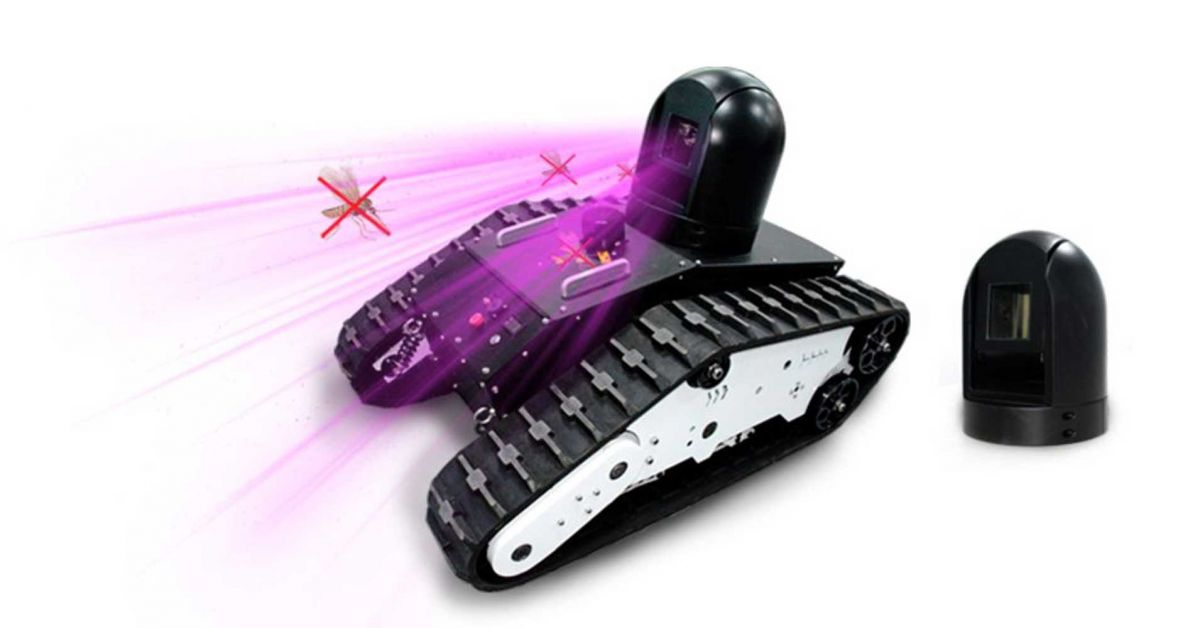
\includegraphics[width=0.8\linewidth]{robot.jpg}
 		
 	\end{figure}
 \end{center}
 
 This robot has been referred to as a toy-sized autonomous mosquito zapper, designed by a company named LeiShen. Although there is not much information on this whether this robot has actually been deployed or what kind of components it uses, this robot is similar to the project's aim.


\subsection{Autonomous Roomba}
  \begin{center}
	
	
	\begin{figure}[H]
		\centering
		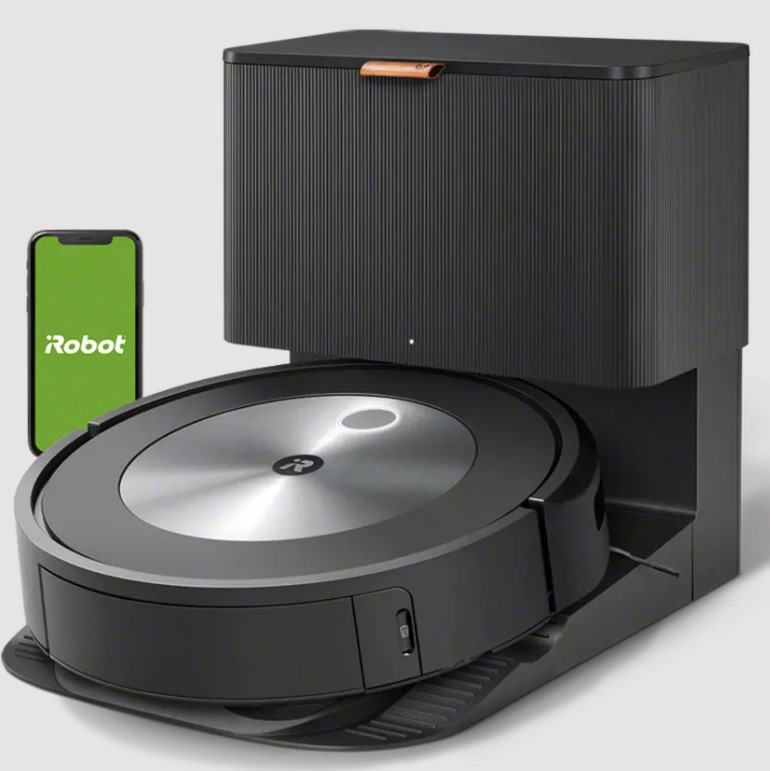
\includegraphics[width=0.46\linewidth]{robot2.jpg}
		
		\label{fig:Robot}
	\end{figure}
\end{center}

Although a robot vacuum is different from a mosquito zapper the concept is similar. This mosquito zapper shoul be able to roam around room autonomously just like the vacuum and avoid obstacles or have a hard encasing to control damage on the hardware. It 



 

 	
 \subsection{Design}
 
 
 
 
 
 	\section{Hardware structure}
 	 
 	
 	\begin{center}
 		
 		
 		\begin{figure}[H]
 			\centering
 			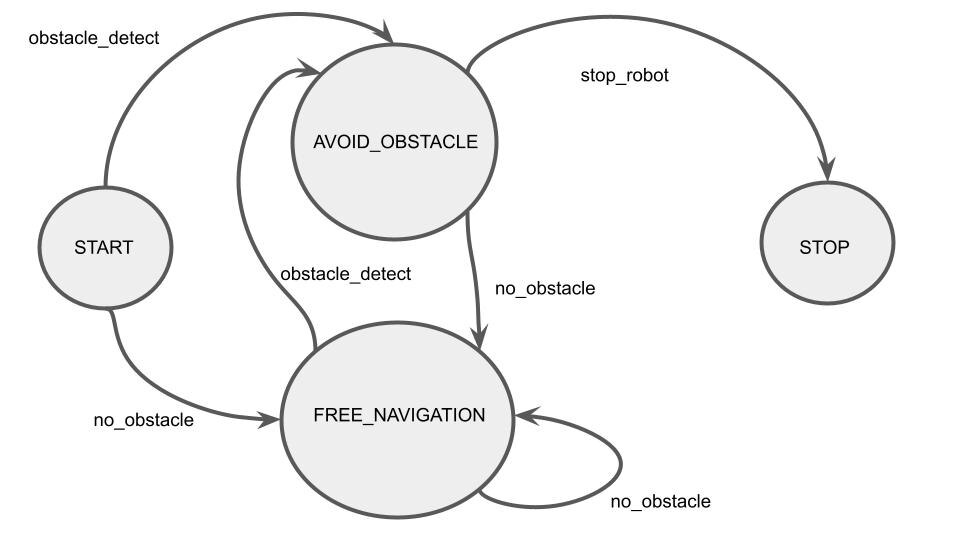
\includegraphics[width=0.6\linewidth]{fsm1.jpg}
 			\caption{An autonomous mosquito zapper robot roaming }
 			\label{fig:robot}
 		\end{figure}
 	\end{center}
 	
 	
 	\subsection{Making the circuit}
 	
 	
 	This section will provide the necessary electrical energy to power the laser, servo motor and other components.
Power supply voltage: The voltage of the power supply will determine the voltage of the electrical energy available to the circuit, and will affect the performance and power consumption of the components in the circuit.

Component voltage ratings: Each component in the circuit will have a rated voltage, which is the maximum voltage that the component can safely handle. You will need to ensure that the power supply voltage and the voltages applied to the components in the circuit are within the rated voltages of the components.

Current ratings: Each component in the circuit will also have a current rating, which is the maximum current that the component can safely handle. You will need to ensure that the current flowing through the components in the circuit is within the rated currents of the components, to prevent damage and overheating.

Resistance and impedance: The resistance and impedance of the components in the circuit will affect the flow of current and the voltage applied to the components. You will need to consider these variables when designing the circuit to ensure that the components are operating within their safe limits.
 
 	 	\subsection{Connecting the Hardware}
 	
 	Connect the camera and other sensors to the control system, using appropriate cables and interfaces. This will allow the control system to receive input from the sensors and use this information to control the robot's movements and laser.
 	
 	Connect the servo motor or robotic arm to the control system, using appropriate cables and interfaces. This will allow the control system to control the movement of the servo motor or robotic arm, and thus aim the laser at the detected mosquitoes.
 	
 	Connect the laser to the control system, using appropriate cables and interfaces. This will allow the control system to control the firing of the laser, and kill the detected mosquitoes on contact.
 	
 	Test the circuit to ensure that all of the components are working together as intended, and make any necessary adjustments or repairs.
 	
 
 	The calculation required to move the servo in an appropriate way to point towards the mosquito is usually dependant on the  design of the robot, however in this project  the location and movement information of the detected mosquito provided by the camera and image processing algorithms will be used to calculate the necessary angle and direction for the servo motor or robotic arm to move the laser.
 	
 	For example, if your robot uses a servo motor to aim the laser, you can use the location of the detected mosquito relative to the center of the camera's field of view to calculate the angle at which the servo motor needs to move the laser. This can be done using basic trigonometry, by calculating the angles formed by the lines connecting the center of the camera's field of view, the location of the detected mosquito, and the servo motor axis.
 	
 	Alternatively, if your robot uses a robotic arm to aim the laser, you can use the location of the detected mosquito in three-dimensional space to calculate the position and orientation of the end effector (the part of the robotic arm that holds the laser) that is required to point the laser at the mosquito. This can be done using inverse kinematics algorithms, which calculate the joint angles of the robotic arm that are necessary to achieve a desired end effector position and orientation.
 	


 	
 
 	
 	
 	
 	







 
 \section{Software}
 
 \begin{center}
 	
 	
 	\begin{figure}[H]
 		\centering
 		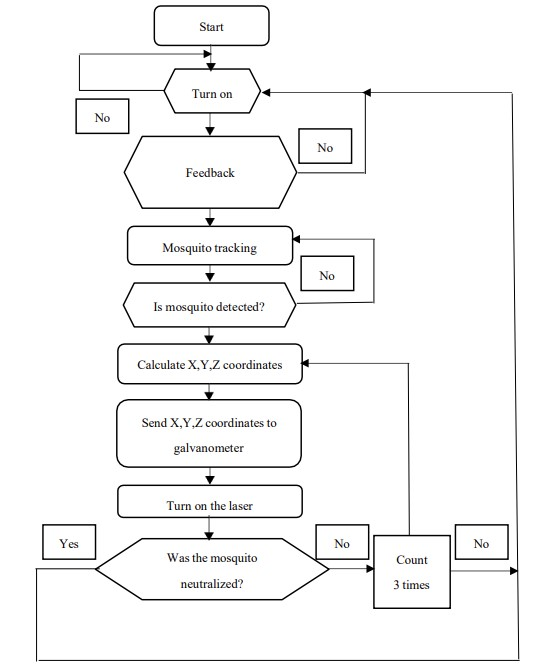
\includegraphics[width=0.8\linewidth]{workinginstallation.jpg}
 		\caption{A flowchart  }
 		\label{fig:Flowchart}
 	\end{figure}
 \end{center}
 

Use image processing algorithms to automatically detect and track mosquitoes in the camera's field of view. This can be done using techniques such as thresholding, edge detection, and object recognition algorithms.

Use the detected mosquitoes to identify their location and movement direction, and use this information to control the robot's movements and aim the laser.

Fire the laser at the detected mosquitoes, using the robot's aiming mechanism, to kill them on contact.


To make the laser move according to the camera, a servo can be used or in a scaled up project robotic arm to aim the laser. In this case the servo motor can be controlled by the robot's control system, using the location and movement information of the detected mosquitoes provided by the camera and image processing algorithms.

For example, the control system can use the location of the detected mosquitoes to calculate the necessary angle and direction for the servo motor or robotic arm to move the laser. This information can then be sent to the servo motor or robotic arm, which will move the laser to the desired position.

Alternatively, you can use a fixed laser and position the camera and servo motor or robotic arm in such a way that the laser is always aimed at the center of the camera's field of view. In this case, the control system can use the movement of the detected mosquitoes to adjust the pan and tilt angles of the camera and servo motor or robotic arm, to keep the laser pointed at the mosquitoes as they move.

Overall, the key to making the laser move according to the camera is to use a control system that can process the location and movement information of the detected mosquitoes, and use this information to control the servo motor or robotic arm that aims the laser.








	

	
	

	\section{Component List}
	\begin{itemize}
		
	\item A mosquito detection system, such as a high-resolution camera or a specialized sensor that can detect the presence of mosquitoes.
	
	\textbf{High-resolution cameras}: A camera with a high frame rate and good resolution can be used to capture images of mosquitoes and identify them based on their shape and size. This can be combined with image processing algorithms to automatically detect and track mosquitoes in real-time.
	
		sensor for detecting mosquitoes will depend on the specific design and requirements of your robot, as well as the environment in which it will be used.
		 	

		

	To detect mosquitoes using a high-resolution camera, you can follow these steps:
	
	Install the camera on your robot, and position it so that it has a clear view of the area where mosquitoes are likely to be present.
	
	Set the camera to a high frame rate and resolution, to capture detailed images of the mosquitoes
	
	
	
	High-resolution camera: A high-resolution camera, such as the Raspberry Pi Camera Module or the Arduino Camera Shield, can be used to detect and track mosquitoes in the robot's field of view.
	
	
	\begin{center}
		\setlength{\tabcolsep}{10pt} % Default value: 6pt
		\renewcommand{\arraystretch}{1.5} % Default value: 1
		\begin{tabular}{ | m{3cm} |m{3cm} | m{4cm}|  } 
			\hline
			Camera  & Price &Function  \\ 
			
			\hline
			FRaspberry Pi High Quality Camera Module
			 & £57 & Function
			
			\\ 
			\hline
			Arduino Camera Shield & £61.00 & function
			\\ 
			\hline
			Stereo Camera & £75 & function.\\ 
			\hline
		\end{tabular}
	\end{center}
	
	
		\textbf{Servo motor or robotic arm}: A servo motor, such as the Tower Pro SG90 or the DYNAMIXEL AX-12A, or a robotic arm, such as the DOBOT Magician or the Dagu Wild Thumper, can be used to aim the laser at the detected mosquitoes.	A mechanism for aiming and firing the laser, such as a \textbf{servo motor} or a robotic arm.
	
	\textbf{Laser}: A laser, such as the 445nm Blue Laser Module or the 532nm Green Laser Module, can be used to kill the detected mosquitoes on contact.	A laser, or other high-intensity light source, that is capable of killing mosquitoes on contact.
	
	\textbf{Control system}: A control system, such as a Raspberry Pi or an Arduino board, can be used to process the input from the camera and other sensors, and control the servo motor or robotic arm and the laser.	A control system, such as a microcontroller or a computer, to process the input from the mosquito detection system and control the laser firing mechanism.
	
	\textbf{Power supply}: A power supply, such as a battery or a plug-in power supply, can be used to provide the necessary electrical energy for the circuit.
		A power source, such as a battery or a plug-in power supply, to provide the necessary energy for the laser and the other components.
	
	
	

	

	

	
\textbf{	A housing or chassis} to hold and protect the other components, and provide a way for the robot to move around and access areas where mosquitoes may be present.
	
	In addition to these core components, you may also need additional hardware and software components, such as sensors for navigation and \textbf{obstacle avoidance}, and software for image processing and control algorithms.
	
	
	
	
		\end{itemize}
		


	

	
	
	
\section{Safety Protocol}

	
	To ensure that your mosquito-detecting robot circuit is connected safely, you can follow these steps:
	
	Use appropriate wiring and connectors for the circuit. This will ensure that the connections are secure and able to withstand the current and voltage levels in the circuit.
	
	Use fuses or circuit breakers to protect the circuit from excessive current. This will prevent damage and potential hazards if there is a short circuit or other electrical malfunction in the circuit.
	
	Use appropriate power supplies and voltage regulators to ensure that the voltage applied to the circuit is within the rated voltages of the components. This will prevent damage and ensure that the components are operating at their optimal levels.
	
	Use appropriate heat sinks and other cooling measures to prevent overheating of the components in the circuit. This will ensure that the components are able to dissipate heat effectively and operate within their safe temperature limits.
	
	Test the circuit before using it, to ensure that it is functioning properly and safely. This can be done using a multimeter or other test equipment to measure the current, voltage, and resistance in the circuit, and verify that the values are within the safe limits for the components.
	
	Overall, by following these steps and using appropriate wiring, connectors, and protective measures, you can ensure that your mosquito-detecting robot circuit is connected safely and functions properly.
	
	
	
	
	


	
	
	\section{Further Development}
	
	
	There are several sensors that can be used to detect mosquitoes, depending on the specific requirements of your robot. Some possible options include:
	
   Developing more advanced algorithms for mosquito detection and tracking. This could involve using machine learning algorithms to improve the accuracy and efficiency of the detection and tracking process, and enable the robot to adapt to different types of mosquitoes and environments.
	
	Enhancing the robot's ability to navigate and avoid obstacles. This could involve using additional sensors, such as lidar or ultrasonic sensors, to enable the robot to map its surroundings and avoid collisions with objects and people.
	
	Improving the robot's power efficiency and battery life. This could involve using more efficient components and algorithms, and implementing power management strategies, to enable the robot to operate for longer periods without needing to be recharged.
	
	Expanding the robot's capabilities to include other functions, such as insecticide application or air quality monitoring. This could involve adding additional sensors and mechanisms to the robot, and developing new algorithms and control systems to support these additional functions.
	
	
	Acoustic sensors: Mosquitoes make distinctive buzzing sounds when they fly, which can be detected using microphones or other acoustic sensors. This type of sensor can be used to detect the presence of mosquitoes, but may not be able to provide precise location information.
	
	Heat sensors: Mosquitoes are attracted to the heat and carbon dioxide produced by warm-blooded animals, including humans. A heat sensor, such as a thermal imaging camera, can be used to detect the presence of mosquitoes by detecting their heat signature.
	
	Chemical sensors: Mosquitoes are attracted to certain chemicals, such as lactic acid and other human perspiration compounds. A chemical sensor, such as a gas chromatograph, can be used to detect the presence of these chemicals and infer the presence of mosquitoes in the area.
	
	
	
	
	\section{Brief Review And Analysis}
	In one similar experiment, found that using OpenCV solely to using a tracker function to track the movement of a mosquito in different methods did not give the greatest results. 
	\begin{center}
		
		
		\begin{figure}[H]
			\centering
			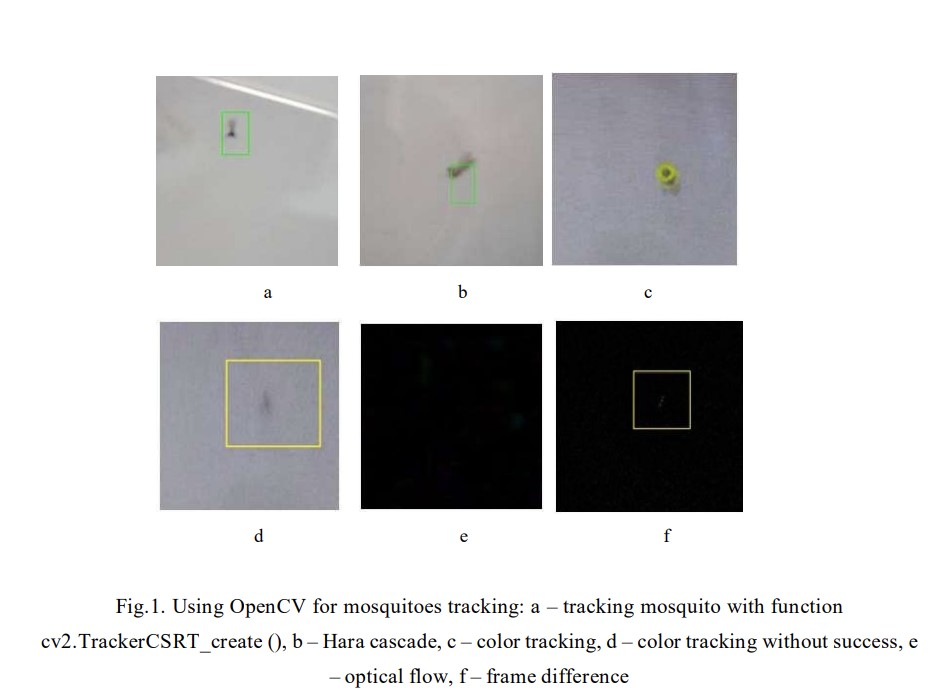
\includegraphics[width=1\linewidth]{opencv.jpg}
			
			\label{fig:opencv}
		\end{figure}
	\end{center}
	As seen in the figure above the mosquito in one of the methods cannot be detected at all, however by using an image processing function called Thresholding ON A 2-4mm sized mosquitoes gave drastically different results:
	
	\begin{center}
		
		
		\begin{figure}[H]
			\centering
			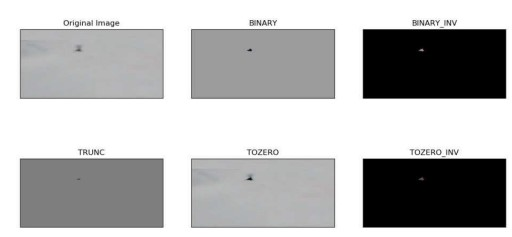
\includegraphics[width=0.8\linewidth]{opencv1.jpg}
			
			
		\end{figure}
	\end{center}
	
	
	
	\section{Conclusion}
	
	
	
	
	\end{document}


